% vim:spell:spelllang=en
\chapter{Register Allocation\Author{F. Bouchez, S. Hack}}
\inputprogress
\label{chap:register-allocation}

{

\newenvironment{important}{%
\bgroup \color{blue!50!black}
  }{
\egroup 
}

%% Local macros for personal use
\newcount\todocount \todocount=0
\def\todo#1{\global\advance\todocount by 1 {\color{blue} {\bf TODO:} #1}}
\newlinechar=`\^^J
\def\endofchapter{\ifnum\todocount>0\immediate\write16{^^JLaTeX Warning: There 
was still TODO macros: \the\todocount.^^J}\fi}


\def\
\def\ac#1{#1}
\def\dom{\preceq}
\def\ssa{SSA\xspace}
\def\maxlive{\ensuremath{\mathrm{Maxlive}}\xspace}
\def\regs{\ensuremath{R}\xspace}
\def\irc{Iterated Register Coalescing\xspace}

\graphicspath{{register_allocation/}{part4/register_allocation/}}

% \chapterauthor{Bouchez, Hack}

Register allocation maps the variables of a program to physical memory locations.
The compiler determines the location for each variable and each program point.
Ideally, as many operations as possible should draw their operands from processor registers without loading them from memory beforehand.
Due to the huge latency of the memory hierarchy (even loading from L1 cache takes three to ten times longer than accessing a register), register allocation is one of the most important optimizations in a compiler. 

There is only a small number of registers available in a CPU, with usual values ranging from~8 to~128.
Hence, the task of register allocation is not only assigning the variables to registers but also deciding which variables should be evicted from registers and when to store and load them from memory (spilling).
Furthermore, register allocation has to remove spurious copy operations (copy coalescing) inserted by previous phases in the compilation process, and to deal with allocation restrictions that the instruction set architecture and the runtime system impose (register targeting).


\section{Introduction}

{\sl
\begin{itemize}
  \item based on graph coloring, linear scan
  \item spilling \& coloring are dependent
  \item heuristics are used to find a working solution
  \item avoiding spills is more important than coalescing
  \item Fab: It is important to outline that with decoupled reg-alloc, spilling and coloring become much simpler and more efficient.
\end{itemize}
}

Register allocation is usually performed per procedure.
A liveness analysis determines for each variable the program points where the variable is live.
A variable is live at a program point if there exists a path from this point on which the variable will be used later on and is not overwritten before that use.
Hence, storage needs to be allocated for that variable; ideally a register.
The set of all program points where a variable is live is called the \emph{live-range} of the variable.
The resource conflict of two variables is called \emph{interference} and is usually defined via liveness:
Two variables interfere if (and only if) there exists a program point where they are simultaneously live.\footnote{
This definition of interference by liveness is an overapproximation.
There are refined definitions that create less interferences.
However, in this chapter we will restrict ourselves to this definition.
}
The number of live variables at a program point is called the \emph{register pressure} at that program point. 
The maximum register pressure over all program points in a procedure is called the register pressure of that procedure, or ``\maxlive.''

It is helpful to think of interferences as an undirected \emph{interference graph:} The nodes are the variables of the program, and two nodes are connected if they interfere.
The set of variables live at some program point form a \emph{clique} in this graph:
Any two variables in this set interfere, hence their nodes are all mutually connected.
The size of the largest clique in the interference graph is called its \emph{clique number}, denoted $\omega$.
A \emph{coloring} of this graph with~$k$ colors corresponds to a valid register allocation with~$k$ registers.
Hence, we will use the terms ``register'' and ``color'' interchangeably in this chapter.
A $k$-coloring is a mapping from the nodes of the graph to the first~$k$ natural numbers (called colors) such that two neighbouring nodes have different colors.
The smallest~$k$ for which a coloring exists is called the \emph{chromatic number}, denoted $\chi$.
Of course $\chi\ge\omega$ holds for every graph, because the nodes of a clique must all have different colors.

Chaitin et al.~\cite{chaitin:1981:register} showed that for every undirected graph, there is a program whose interference graph is this graph.
From the NP-completeness of graph coloring then follows the NP-completeness of register allocation.
Hence, determining the chromatic number of an interference graph is not possible in polynomial time unless P=NP.

This the major nuisance of classical register allocation:
The compiler cannot efficiently determine how many registers are needed.
This means one might need more registers than \maxlive, \maxlive being only a lower bound on the chromatic number.
The somewhat unintuitive result is that, even if at every program point there are no more than \maxlive variables live, we still might need more than $\maxlive$ registers for a correct register allocation!
The causes of this problem are control-flow merges, %since they create cycles in the interference graph,
as can be seen in Figure~\ref{fig:ra:exprg}.

\begin{figure}[htbp]
	\begin{center}
		\subfigure[Example program and live-ranges of its variables]{ 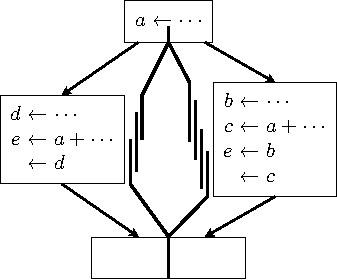
\includegraphics{figures/prog_lr.pdf}
                \label{sub:ra:exprg:prog}
                }
		\qquad
		\subfigure[Interference graph]{ 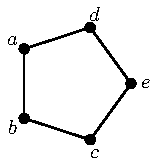
\includegraphics[scale=1.1]{figures/prog_ig.pdf} }
	\end{center}
	\caption{Example program and its interference graph}
	\label{fig:ra:exprg}
\end{figure}

In that example, the register pressure is at most two at every program point.
However, the interference graph cannot be colored with two colors. 
Its chromatic number is three.
The inequality between \maxlive and the chromatic number is caused by the cycle in the interference graph.\footnote{
In theory, the gap between the chromatic number and \maxlive can even be arbitrarily large.
This can be shown using by applying Chaitin's proof of the NP-completeness of register allocation to Mycielski graphs.}

This situation changes if we permit \emph{live-range splitting.} That is, inserting a copy (move) instruction at a program point that creates a new variable.
Thus, the value of the variables is allowed to reside in different registers at different times.
In Figure~\ref{sub:ra:exprg:prog}, assume we split the live-range of~$e$ in the left block: we rename it by~$e'$ and add a copy~$e \gets e'$ at the end of the block.
Then, the node~$e$ in the graph is split into two nodes, $e$ and~$e'$, that do not interfere: this breaks the cycle in the graph, making its chromatic number equal to two, i.e., \maxlive.
%(cf.~the SSA version of the program shown in Figure~\ref{fig:ra:exprgssa}).

% \begin{figure}[htbp]
% 	\begin{center}
% 		\subfigure[Example program with live-range of~$e$ split]{ 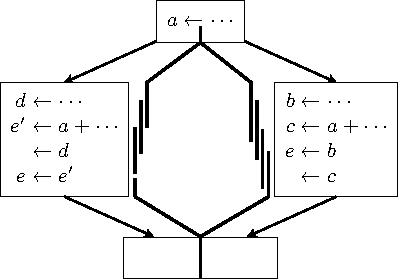
\includegraphics{figures/prog_split_lr.pdf} }
% 		\qquad
% 		\subfigure[Interference graph]{ 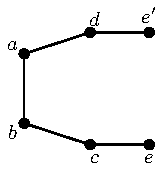
\includegraphics[scale=1.1]{figures/prog_split_ig.pdf} }
% 	\end{center}
% 	\caption{Example Program with spit live-range and its interference graph}
% 	\label{fig:ra:exprgsplit}
% \end{figure}

In an extreme setting, one could split the live-ranges of all variables after every instruction.
The interference graph degenerates into several disconnected components and its chromatic number drops to \maxlive.
Of course, such an extreme live-range splitting introduces \emph{a lot} of shuffle code, which degrades the runtime of the compiled program.
This interplay between live-range splitting and colorability is the key issue in register allocation.

\subsection{Non-SSA Register Allocators}
As finding a valid $k$-coloring is NP-complete, assigning registers is performed by some heuristic algorithm.
If that algorithm fails to assign a register to a variable, then it either spills this variable to memory, or frees a register by spilling the variable it contains.
The problem here is that the spilling decision is made to revive the coloring heuristic, and not because the variable that gets spilled is in itself a good candidate for spilling. 
Even worse, we might spill a variable because the heuristic is ``not good enough,'' and not because we are actually out of registers.

At the same time, classical algorithms perform copy coalescing (i.e.,~undoing live-range splitting) during coloring.
However, if done aggressively, coalescing may increase the chromatic number of the graph, or make the graph harder to color for the heuristic.
Both cases generate additional spills.
This is of course unacceptable because we never want to add memory accesses in favor of an eliminated copy.
Thus, existing techniques often apply \emph{conservative} coalescing approaches which are guaranteed not to increase the chromatic number of the graph, at the expense of the quality of the coalescing.

\subsection{SSA form to the rescue of register allocation}

The live-ranges in an SSA form program all have a certain property:
SSA requires that all uses of a variable are dominated by its definition.
Hence, the whole live-range is dominated by the definition of the variable.
Dominance, however, induces a tree on the control-flow graph.
Thus, the live-ranges of SSA variables are all tree-shaped~\cite{Bouchez05:RR,brisk:2006:poly,HGG:2006:RA_SSA}.
They can branch downwards on the dominance tree but have a single root:
the program point where the variable is defined.
Hence a situation like in Figure~\ref{fig:ra:exprg} can no longer occur:
$e$~had two ``roots'' because it was defined twice.
Under SSA form, the live-range of~$e$ is split by a \phifun.
The argument and result variables of that \phifun constitute new live-ranges, giving more freedom to the register allocator since they can be assigned to different registers.

\begin{figure}[htbp]
	\begin{center}
		\subfigure[example program in SSA]{ 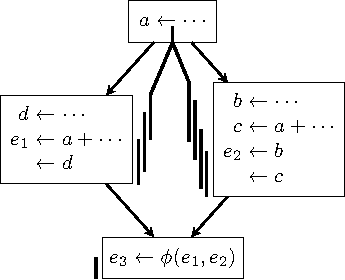
\includegraphics{figures/prog_ssa_lr.pdf} }
		\qquad
		\subfigure[Interference graph]{ 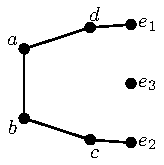
\includegraphics[scale=1.1]{figures/prog_ssa_ig.pdf} }
	\end{center}
	\caption{SSA version of the example program}
	\label{fig:ra:exprgssa}
\end{figure}

This special structure of the live-ranges leads to a special class of interference graphs:
Gavril~\cite{gavril:1974:trees} showed that the intersection graphs of subtrees are the \emph{chordal graphs}.
Chordal graphs can be optimally colored in linear a time with respect to the number of edges in the graph.
Furthermore, they are \emph{perfect}, which means that for every subgraph, the clique number equals the chromatic number. 
This is a very important property for register allocation because it means that \maxlive equals the chromatic number of the graph;\footnote{
This also implies that chordal graphs do not have ``holes'' like the interference graph in Figure~\ref{fig:ra:exprg}.
Every cycle is spanned by \emph{chords.}
}
It has even been shown~\cite{Bouchez05:RR,HGG:2006:RA_SSA} that, for every clique in the interference graph, there is one program point where all the variables of that clique are live.
This allows to decouples spilling from coloring:
First, lower the register pressure to~$k$ everywhere in the program;
Then, color the interference graph with~$k$ colors in polynomial time.


\section{Spilling}

The term spilling is heavily overloaded:
In the graph-coloring setting it often means to spill a node of the interference graph and thus the \emph{entire} live-range of a variable.
This implies inserting load instructions in front of every use and store instructions after each definition of the (non-SSA) variables.
Other approaches, like some linear scan allocators, are able to keep parts of the live-range of a variable in a register such that multiple uses can potentially reuse the same reload.

\subsection{Spilling under the SSA Form}

As stated above, lowering \maxlive to~\regs ensures that a register allocation with \regs registers can be found in polynomial time for SSA programs.
Thus, spilling should takes place before registers are assigned \emph{and} yield a program in SSA form.
For the moment, let us ignore \emph{how} to choose ``what'' to spill and ``where,'' and concentrate on the implications of spilling in SSA programs.
Because many compilers use SSA heavily, it is a reasonable assumption that the program was in SSA before spilling.
Hence, we consider spilling as an SSA program transformation that establishes $\maxlive\le\regs$ by inserting loads and stores into the program.


\subsection{Finding Spilling Candidates}

How to find program points to place loads and stores such that $\maxlive\le\regs$?
Let us start with a simplistic setting where the location of loads and stores is not optimized:
loads are placed directly in front of uses and stores directly after the definition.
Furthermore we consider a \emph{spill everywhere} setting:
a variable is either spilled completely or not at all;
If spilled, the live-range of a variable then degenerates into small intervals: one between the definition and the store, and one between each load and its subsequent use.
\todo{figure? Flo: if space allows it, yes.}
Gavril and Yannakakis~\cite{YannakakisGavril87} showed that, even in this simplistic setting, it is NP-complete to find the minimum number of nodes to establish $\maxlive\le\regs$.
Bouchez et al.~\cite{BouchezDR07:spill} showed that it is even NP-complete to find the minimum number of nodes to spill to decrease \maxlive just by one.
Thus, finding spill candidates is not facilitated by SSA.


Moreover, formulations like \emph{spill everywhere} are often not appropriate for practical purposes,
and putting the whole live-range to memory is too simplistic.
A variable might be spilled because at some program point the pressure is too high;
However, if that same variable is later used in a loop where the register pressure is low,
spilling everywhere will place a superfluous (and costly!) load in that loop.
Spill everywhere approaches try to minimize this behavior by adding costs to variables;
These bring in a flow-insensitive algorithm information that a variable reside an frequently executed area.
However, such approximations are often too coarse to give good performance.
Hence, it is imperative to intelligently split the live-range of the variable according to the \emph{program structure} and spill only parts of it.

More promising spilling techniques are based on Belady's algorithm~\cite{belady:1966:storage}.
Belady's algorithm was developed in the context of page replacement in operating systems;
When all pages slots are used a new page must be mapped in, the question is: ``which page to evict?''
Each time this question arise, a different page might be chosen;
If an evicted page was brought back, it is not necessarily evicted again.
This problem is very similar to register allocation, besides the fact that \emph{putting} a register to memory (evicting a page) also incurs a cost (a store) in the register allocation setting while it does not in the page replacement setting.
Belady showed that evicting the page whose next use is farthest in the future leads to the minimum number of page loads. 
Nevertheless, Farrach and Liberatore~\cite{farach:98:local} showed that Belady's algorithm gives good results on straight-line code.

Braun and Hack~\cite{BH:2009:Spill} extended Belady's algorithm to general control-flow graphs in two ways.
First, they gave a data-flow analysis to compute approximate next use values on the control-flow graph.
In this next use calculation, loops are virtually unrolled by a large factor such that code ``behind'' loop appears far away from code in front of the loop.
This forces the eviction algorithm to prefer variables that are not used in loops and to leave parts of live-ranges that are used within loops in registers.
Second, they showed how and in which order to process the basic blocks of the control-flow graph in order to determine a reasonable initial register occupation for each block.

\subsection{Maxlive and colorability of graphs}
\todo{seb: do we need this? doing  a standard liveness analysis does the job. we can also refer to Appel's liveness algo.}

{\sl
\begin{itemize}
  \item definition of Maxlive
  \item show that Maxlive is the minimum number of colors required
  \item scan of the dominance tree sufficient to know Maxlive: pseudo-code
  \item Fab: MAXLIVE minimum if interference graph==intersection graph. Clearly we do not want to go into such details but be careful to use precise and correct terms.
\end{itemize}
}
    
The register pressure at a program point is the number of variables alive at 
this point.\footnote{Considering all simultaneously alive variables interfere.}
The greatest register pressure over all a program is called \maxlive, 
since it is the maximum number of simultaneously alive variables. Obviously, 
spilling is mandatory if \maxlive is strictly greater than $R$, the number of 
registers.
Under SSA, the good news is that this is the only case where spilling is 
required, i.e., if \maxlive $\leq R$, there is no need for spilling. Indeed, 
\maxlive is the coloring number of the chordal interference graph of the 
program (\todo{ref to chapter 2?}). So, we can devise a polynomial test to know 
whether spilling is necessary or not by computing \maxlive. This can be done by 
checking on every program point the number of variables that are alive. If 
liveness information is available on the whole program, the order does not 
matter. However, in the case of SSA, this is not required as \maxlive can 
easily be computed without liveness information by performing a scan of the 
dominance tree, starting from the root. We only need to know which uses are 
``last-uses.'' The pseudo-code is given on Figure~\ref{code:compute-maxlive}.
\todo{check \maxlive scan needs last uses}.


\begin{figure}[ht]
  \begin{verbatim}
  function compute-branch (p, live)
    live <- live - { uses in p that are last uses }
    live <- live + { definitions of p }
    maxlive <- max( maxlive, #live )
    foreach child c of p
      compute-branch (c, live)

  function compute-maxlive
    maxlive <- 0
    compute-branch (root, {})
  \end{verbatim}
  \caption{Pseudo-code for \maxlive}
  \label{code:compute-maxlive}
\end{figure}





\section{The problem of spilling}
\subsection{Lowering Maxlive}

{\sl
\begin{itemize}
  \item The min number of colors is Maxlive. Variables must be stored in memory 
    to lower the register pressure at points where it is $>R$.
  \item Whenever, Maxlive $\leq R$, we know for sure that spilling more in 
    unnecessary.
  \item Fab: if MAXLIVE$\leq R$ spilling is unecessary under some conditions (we color SSA code, going out of SSA code might require some additionnal spilling. Also without naming constraints). So again be careful about what you say. I think that the idea is to have a register allocator under SSA as simple as possible with a very simple modeling and nice properties. Then we cope with real world issues during the colored-SSA destruction.
\end{itemize}
}

Usually, there are too many variables in a program and \maxlive is greater than 
$R$. In that case, we need to lower the register pressure at program points 
where it exceeds $R$ by spilling, i.e., storing variables in memory instead of 
registers. Whenever we reach a point where \maxlive $\leq R$, it will be 
possible to color all SSA variables with the $R$ registers. For now, the 
difficulty lies in choosing which variables to spill, and where to spill them. 
Indeed, a careful choice will lead to performance, while making bad decisions 
can lead to big slowdowns. As accesses to variables in memory require more time 
that accesses to registers, it is for instance better to avoid spilling 
variables used inside frequently executed code regions like loops.

\todo{spilling while keeping SSA property}


\subsection{Spilling is a difficult problem}

The problem of spilling is a difficult one in the literature, even under one of 
its simpler forms, the spill everywhere problem, where spilled variables stay 
so on their entire live-range~\cite{todo}. This spilling is advocated on the 
first graph-coloring algorithms~\cite{chaitin:1981:register} and even in subsequent 
algorithms~\cite{IRC} because it fits better the graph-coloring representation. 
In these schemes, this amounts to removing nodes from a non $R$-colorable graph 
until it becomes $R$-colorable. Although this node deletion problem is known to 
be NP-complete, this allows the writing of simple heuristics based on the 
number of neighbours in the graph and a cost attached to nodes representing the 
overhead incurred in case they were to be spilled. An added problem is the fact 
that, for many architectures like RISC, spilled variables cannot be accessed 
directly from memory but must instead by copied back to the registers, when 
they are used, or which must be in a register when defined, just before being 
copied to memory. This creates new variables with very short live-ranges at the 
definition and use points, which must be accounted for register allocation. 
This explains why algorithms such as \irc must rebuild the interference graph 
after a phase of spilling and start again, until no more spilling is required.


The actual spilling problem is even more difficult, as variables do not have to 
be spilled on their entire live-range.
% borrowed from sebastian's CC'09 paper
Consider a loop with excessive register pressure and a variable that is defined 
before the loop and used afterwards. Ideally, a compiler would store (spill) 
the variable in front of the loop and load (reload) the variable after the 
loop. If the variable was reloaded inside the loop, the reload would be 
executed in each loop iteration. Another example is a variable that is used in 
a loop but has already been spilled before the loop. Reloading this variable 
directly before its use in the loop will cause memory traffic in each loop 
iteration. Thus, it is preferable to put the reload in front of the loop.
% end of borrowing
This poses a new problem on top of choosing which variables to spill: now we 
need also to choose where to spill them, i.e., where to put {\tt load} and {\tt 
store} instructions. This more general problem where the goal is to minimize 
the overhead of these added instructions is called the load-store optimization 
problem and is known to be NP-complete, even for a 
basic-block~\cite{Liberatore00}.  


\subsection{SSA does not help for spilling}
{\sl
\begin{itemize}
  \item easy spill method: spill everywhere
  \item SSA split points are good for coloring, but not really for spilling 
    (see article spill everywhere under SSA)
  \item other split points to avoid spill everywhere are probably better
  \item Fab: if you need an example to illustrate that SSA does not really help 
    in practice for spilling ask Quentin. It does help a little bit (dynamic 
    programming possible for spill everywhere with few registers; further first 
    can be generalized). But what you want to point it here is the fact that 
    the disadvantages seem more important than advantages.
  \item Fab: the LCTES spill everywhere article does not discuss practical issues (such as the fact that it might insert a load or a store inside a loop...). It is more algorithmical issues.
  \item Seb: Want do we want to say here?
  	  I think the title of the section is too negative. 
  	  Perhaps we should merge the section with the last.
  	  I think it would be good to first talk about different definitions for spilling,
  	  then give an overview over your results (LCTES paper).
\end{itemize}
}

For the spilling problem, the SSA is not really of much help. Over a blind 
spill everywhere algorithm on the initial program, it has however the slight 
advantage of allowing the spilling of SSA variables, i.e., sub-variables of the 
initial variables. One major disadvantage is the added complexity when spilling
variables defined in \phifuns \todo{explain the problem if not all args are 
spilled, or if spilled in $\neq$ locations}.
\todo{Seb: complexity? perhaps slight complications :)}

{\sl Examples by Quentin}
\begin{minipage}{.45\textwidth}
\begin{verbatim}
CSSA :
   a =
   b =
 /       \
c= a   d = b
 \       /
 e = phi(c,d)
 = e
\end{verbatim}
\end{minipage}
\begin{minipage}{.45\textwidth}
After spilling spill :
\begin{verbatim}
   a =
   b =
 /          \
c= a     d = b
C=st c  D = st d
 \          /
 E = phi(C,D)
 e = ld E
 = e
\end{verbatim}
\end{minipage}
In that case, memory locations C, D and E can be the same. But this does not 
mean that placement of {\tt store} instruction is the best one.

\begin{minipage}{.45\textwidth}
\begin{verbatim}
SSA :
   a =
   b =
 /         \
 \         /
 e = phi(a,b)
 = e
\end{verbatim}
\end{minipage}
\begin{minipage}{.45\textwidth}
Spill supposing {\tt store}s are after definition
\begin{verbatim}
   a =
   A = st a
   b =
   B = st b
 /         \
 \ <--     / <--
 E = phi(A,B)
 e = ld E
 = e
\end{verbatim}
\end{minipage}

On the two edges pointed by arrows (or on the preceding basic block if they are 
not critical), additional memory transactions must reconcile the values:
\begin{verbatim}
tmp = ld X
Y = st tmp
\end{verbatim}

This can induce more spill, unforeseen.
Without SSA, this problem does not exist: for instance, with spill everywhere, 
the same memory slot is affected to all definitions of the same variable so no 
post-treatment is required as it is under SSA.



\subsection{Spilling under SSA}
Still, we give a possibility to perform spilling under SSA
\begin{itemize}
  \item Hack's algorithm: simplified version?
  \item \`a la Belady following dominance tree?

  \item Fab: The last Algorithm from Sebastian is Belady like. So yes try to simplify it, provide the pseudo code and give the intuitions on how the full version improves it.
  \item Seb: I think it's ok to briefly outline the approaches that are out there and refer to the papers.

\end{itemize}
\todo{Ask Sebastian to do it.}


\cite{Braun09:spilling-ssa}\todo{file braun09cc.pdf in biblio}


\section{Coloring and coalescing}

Due to the decoupled register allocation and the use of SSA, the interference graph after spilling has two interesting properties.
First, it still is chordal, hence easily colorable in linear time;
Second, we know that $R$~colors are sufficient to color it since $\maxlive \leq R$.
In this section, we will first present the traditional graph coloring heuristic of Chaitin et al.\ and show how it successfully color programs under SSA form.
We will then present a lighter coloring algorithm based on the scanning on the dominance tree.
Finally, we will then explain how to add \emph{coalescing} to the coloring phase to reduce the number of copies in a program.

 

\subsection{Greedy coloring scheme}
\label{sec:regalloc:greedy-col}

{\sl
\begin{itemize}
  \item two simplicial nodes
  \item color in the reverse order of simplification
  \item one such order considers subtrees from the root of the tree
  \item no need to construct interference graph
  \item Fab: make it as more intuitive as possible. Avoid as much as possible 
    chordal stuffs which are useless. Greedy coloring and its relationship with 
    the subtree representation is important on the other hand. See with Philip 
    to avoid redundancies between your chapter and his (SSA properties). It is 
    important to outline here that this property that is due to decoupled+SSA 
    enables more aggressive coalescing heuristics. But also simpler 
    (tree-scan).
\end{itemize}
}


In traditional graph coloring register allocation algorithms, the assignment is done by coloring the interference graph with the greedy heuristic of Chaitin et al.~\cite{chaitin:1981:register}.
This scheme is based on the observation that given $R$ colors---representing the registers---, if a node in the graph has at most $R-1$ neighbours, there will always be one color available for this node whatever colors the remaining nodes have.
Such a node node can be \emph{simplified}, i.e., removed from the graph and placed on a stack.
This process can be iterated with the remaining nodes, whose degree may have decreased if the simplified node was one of their neighbours.
If the graph becomes empty, we know it is possible to color the graph with $R$ colors; 
Such a coloring can be obtained by assigning colors to nodes in the reverse order of their simplification, i.e., by popping nodes from the stack and assigning them one available color, which is always possible since they have at most $R-1$ colored neighbours.
We call this algorithm the \emph{greedy coloring scheme}.

Since it is a coloring heuristic, this scheme can get stuck (whenever all remaining nodes have degree at least $R$).
In that case, we do not know whether the graph is $R$-colorable or not.
In traditional register allocation, this is the trigger for spilling some variables so as to unstuck the simplification process.
However, we will see that under the SSA form, after spilling has already been done so that the register pressure is at most $R$, the greedy coloring scheme can never get stuck.

\begin{comment}
\begin{function}[h]
\captionlabel{\labelkgreedy}{Is\_kGreedy}{($G$)}
\KwData{Undirected graph $G=(V,E)$; $\forall v\in V$, degree[$v$] = \#neighbours 
of $v$ in $G$, $k$ number of colors}
% \lForEach{$v\in V$}{set degree[$v$] to degree of $v$ in $G$ \;}
stack = $\emptyset$ ;
$\mbox{worklist} = \{ v \in V \mid \mbox{degree[$v$]} < k\}$ \;
\While{$\mbox{worklist} \neq \emptyset$}{
  \KwLet $v \in \mbox{worklist}$ \;
  \ForEach{$w$ neighbour of $v$}{
     degree[$w$] \<- degree[w]-1 \;
     \lIf{$\mbox{degree[$w$]} = k-1$}{worklist \<- $\mbox{worklist} \cup \{w\}$}
  }
  push $v$ on stack ;
  worklist \<- $\mbox{worklist} \setminus \{v\}$  \tcc*{Remove $v$ from  $G$}
}
\lIf{$V = \emptyset$}{\Return{\KwTrue}}
\lElse{\Return{\KwFalse}}
\end{function} 
\end{comment} 

\begin{figure}
\begin{verbatim}
Function Simplify(G)
  Data: Undirected graph G = (V, E);
  For all v, degree[v] = #neighbours of v in G,
  k number of colors
stack = {} ;
worklist = {v in V | degree[v] < k} ;
while worklist != {} do
  let v in worklist ;
  foreach w neighbour of v do
    degree[w] = degree[w]-1 ;
    if degree[w] = k - 1 then worklist = worklist U {w}
  push v on stack ;
  worklist = worklist \ {v} ; /* Remove v from G */
if V != {} then Failure ``The graph is not simplifiable''
return stack ;
\end{verbatim}
\caption{Iskgreedy function}
\label{code:is-k-greedy}
\end{figure}



\subsection{SSA graphs are colorable with a greedy scheme}
\label{sec:regalloc:ssa-greedy}

One of the interesting properties of SSA form for register allocation is that the live-ranges of variables are subtrees of the dominance tree (see Chapter~\ref{chap:properties-and-flavours}, Section~\ref{part1:ssaprop:subtrees}).
This means the interference graph is chordal and can be represented as the intersection graph of a family of subtrees.
We will now prove that if the register pressure is at most $R$, the interference graph can be colored with $R$ colors using the greedy scheme.

\begin{proof}
  Let us consider such a subtree representation of the interference graph (see Figure~\ref{fig:regalloc:subtree} TODO) and try to apply the greedy coloring scheme to it.
  In this representation, a node candidate for simplification corresponds to a live-range which intersect with at most $R-1$ other live-ranges.
  Consider the ``leaf'' of a branch of the dominance tree, i.e., the live-range on this branch which starts last, say at point $d$ (the instruction that defines the leaf).
  If this leaf does not intersect any other live-range, it can be simplified.
  If it does, then all its neighbour live-ranges start before $d$---by definition of the leaf---and end after $d$---because they intersect.
  So, all neighbours of the leaf are live at $d$;
  Since spilling has already been done, we know that the register pressure at $d$ is at most $R$, hence there is at most $R-1$ intersecting live-ranges:
  the corresponding node in the interference graph has at most $R-1$ neighbours and can be simplified.
  Removing a live-range does not change the shape of the graph (the remaining live-ranges are still subtrees of the dominance tree):
  as long at the graph is not empty, there will still be ``leaf'' live-ranges, i.e., nodes that can be simplified.
  Eventually, the simplification process will empty the whole graph, and colors can be assigned in the reverse order of the simplification.
\end{proof}

\begin{figure}
  Insert subtree figure HERE.
  \caption{Subtree}
  \label{fig:regalloc:subtree}
\end{figure}

We just proved that if we are under SSA form and the spilling has already been done so that $\maxlive \leq R$, the classical greedy coloring scheme of Chaitin et al.\ is \emph{guaranteed} to perform register allocation with $R$ without any additional spilling.
This is practical for instance when working on an existing compiler that uses classical register allocation (for instance, the Iterated Register Coalescing of George and Appel~\cite{george:96:iterated}).


The original simplification scheme of Chaitin et al.\ does the job, without any modification. 
Following a call to Is\_k\_Greedy, it is possible to re-use the stack to assign the colors by making a call to Assign\_colors, Figure~\ref{code:assign-color}. 
Among the good things, this also means that existing register allocators can be easily modified to handle SSA code and that register allocation can benefit from powerful coalescing strategies such as aggressive or conservative ones. 
Moreover, the fact that register allocation can be decoupled into a phase of spilling first and then a phase of coloring/coalescing allows the writing of more involved coalescing \todo{cite examples}.


However, this algorithm still needs the interference graph, an additional structure that takes time to build and uses memory up.
We will propose next a lighter coloring algorithm based on the insight given by the greedy coloring scheme.





\begin{figure}
\begin{verbatim}
Function Assign_colors(G)
  available = new array of size R and values True
  while stack != {} do
    v = pop stack ;
    for each neighbour w in G
      available[color(w)] = False
    col = 0;
    for each color c from 1 to R
      if available[c]
        col = c
      available[c] = True /* prepare for next round */
    color(v) = col
    add v to G
\end{verbatim}
\caption{Assign\_color function}
\label{code:assign-color}
\end{figure}



\subsection{A light tree-scan coloring algorithm}
{\sl
\begin{itemize}
  \item On the dominance tree, possible to scan from top and assign colors to 
    variables as they come.
  \item Biased coloring is used to coalesce variables linked by \phifuns.
  \item see next section for more involved coalescing
  \item Fab: I think that you already talked about scan coloring. Ok to talk about biased.
  \item Fab: You can talk about biased coloring that uses the result of an aggressive coalescing (see with Quentin). It is not more complicated and it improves results.
\end{itemize}
}

One of the advantages of SSA is to make things simpler, faster, and use less memory. 
For the register assignment problem, we have seen that the existing greedy scheme based on simplification still works; 
However, it requires constructing and maintaining an interference graph, a structure judged to big and cumbersome to be used in a JIT context, where compilation time and memory prints matter more. 
%This is one of the reasons linear-scan allocators are being developed, even if their performance does not equal those of aggressive time-consuming off-line compilers. 
We will now present a method to perform a fast register assignment for SSA after spilling which does not need more than the dominance tree and def-use chains. 

The algorithm we propose scans the dominance tree, coloring the variables from the root to the leaves in a top-down order.
The variables are colored in the order of their definitions.
A pseudo-code is given in procedure Tree\_Scan, Figure~\ref{code:assign-tree-scan}.
Intuitively, this method works because when the scanning arrives at the definition of a variable, the only colored variables are ``above'' it and since there is at most $R-1$ other variables live at the definition, there is always a free color.
We will now prove that this method always work;
The key observation is that the order in which variables are considered corresponds to a reverse order of simplification, i.e., a valid order of the nodes on the stack after the greedy simplification scheme.

\begin{proof}
  \def\order{o}
  Let us consider an ordering $v_1, v_2, \ldots, v_n$ of the nodes of the nodes based on the dominance:
  if $v_i$ dominates $v_j$, then $v_j$ appear before $v_i$ in the ordering ($j < i$).
  We will show that this order correspond to a greedy simplification.
  Suppose $v_1, \ldots, v_{i-1}$ have been simplified by the greedy scheme (for $i=1$, this is the initial graph).
  If $v_i$ dominates any variable, say $v_j$, then $j < i$ and the node has already been simplified;
  So, there is no variable defined after $v_i$ on the dominance tree:
  the live-range of $v_i$ is a ``leaf'' of the subtree representation (see proof in Section~\ref{sec:regalloc:ssa-greedy}).
  So, $v_i$ can be chosen for simplification, and by induction the ordering $v_1, \ldots, v_n$ is a valid order of simplification. 
  As we have seen previously in Section~\ref{sec:regalloc:greedy-col}, this means the reverse order $v_n, v_{n-1}, \ldots, v_1$ is a valid order for coloring.
\end{proof}


\begin{important}
It is important to understand why this method does not work in the general non-SSA case.
Under SSA, the variables are ``split'' at join points by the use of \phifuns.
If this was not the case, we would have live-ranges that spans on multiple branches of the dominance tree, creating cycles in the representation.
In that case, coloring a branch would constrain the coloring on leaves on a different branch; Under SSA form, such live-ranges are split and their colorings are independent.
See Figure~\ref{TODO} for an example.
\end{important}


\begin{figure}
  \begin{verbatim}
Tree_Scan(T)

  function assign_color(p, available)
    for each v last use at p
      available[color(v)] = True     /* colors not used anymore */

    for each v defined at p
      c = choose_color(v, available)  /* choose available color */
      available[c] = False
      color(v) = c

    for each child p' of p
      assign_color(p', available)

  assign_color(root(T), [True, True, ..., True])

  \end{verbatim}
  \caption{Tree scan coloring algorithm for SSA.}
  \label{code:assign-tree-scan}
\end{figure}


The tree-scan coloring algorithm is really fast as it only needs one traversal of the dominance tree. 
Since the number of colors is fixed and small, it can be implemented as a bit-set to speed-up updates of the {\tt available} array.
The pseudo-code for function {\tt choose\_color} is deliberately not given yet. 
A very basic implementation could just scan the {\tt available} array until it finds one that is not taken.
We will see in the next section how to bias the choosing of colors so as to perform some coalescing. 
 


\subsection{Coalescing under SSA form}

The goal of \emph{coalescing} is to minimize the number of register-to-register {\tt move} instructions in the final code.
While there may not be so many such ``copies'' at the high-level (e.g., instruction ``{\tt a = b;}'' in C)---especially after a phase of copy propagation under SSA (\todo{See chapter X})---,
many such instructions are added by different compiler phases by the time compilation reaches the register allocation phase.
For instance, adding copies is a common way to deal with register constraints (see Section~\ref{sec:practical-regalloc}). 
An even more obvious and unavoidable reason in our case is the presence of \phifuns due to SSA form. 
Indeed, remember that a \phifun represents in fact parallel copies on incoming edges of basic blocks. 
For instance, if the function is $a \gets \phi(b,c)$, then it means that instructions $a\gets b$ should be executed on the edge coming from the left, and $a\gets c$ on the one from the right. 
Suppose now that register allocation decided to put $a$ and $b$ in register $R_1$, but $c$ in register $R_2$;
Then, the copy $a\gets b$ does not need to be executed anymore, but $a\gets c$ still does:
the value of variable $c$ will be contained in $R_2$ and needs to transfered to $R_1$, which means the final code will contain an instruction ``{\tt mov $R_1, R_2$}'' or the like. 



In the case of SSA, it is for instance obviously better to assign variables linked by a \phifun, to the same register, so as to remove copies between subscripts of the same variable ($a_1$, $a_2$, etc.).
This is possible if we are under CSSA, but optimizations can break this property and interferences can appear between subscripted variables with the same origin.
In order to bypass this problem and also allow for more involved coalescing between SSA variables of different origin, we will define a notion of \emph{affinity}, acting as the converse of the relation of interference and expressing how much two variables ``want'' to share the same register. 
We add a metric to this notion, measuring the benefit one could get if the two variables are assigned to the same register.
Given two variables $a$ and $b$, the weight of the affinity between them is the number of occurrences of copy instructions involving them ($a\gets b$ or $b\gets a$) or \phifuns ($a\gets\phi(\ldots,b,\ldots)$ or $b\gets\phi(\ldots,a,\ldots)$). 
These numbers should of course be weighted as a copy in a loop costs more than one outside a loop for instance.
We recommend using using actual execution frequencies based on profiling in possible, and empirically parameters if not
(e.g., $\times 10$ for each level of nested loop, $\times 0.5$ if in a conditional branch, etc.).


\subsubsection{Biased coalescing}

Since the number of affinities is sparse compared to the number of possible pairs of variables, we propose to keep for each variable $v$ an ``affinity list'' where each element is a pair $(u,w)$ meaning that $v$ has an affinity with $u$ of weight $w$.
We propose a version of function {\tt choose\_color} that bias the choosing of colors based on these affinity lists, shown on Figure~\ref{code:choose-color}. 
The bias is very simple, each choice of color maximizes locally, under the current knowledge, the coalescing for the variable being colored. 
It is not of course optimal since the general problem of coalescing is NP-complete~\cite{BouchezDR07:coalescing-cplx}, and biased algorithms are known to be easily misguided. 


\begin{figure}
  \begin{verbatim}
global variables
  count = array of size #colors and elements 0

choose_color(v, available)
  for each (u,weight) in affinity_list(v)
    count[color(u)] += weight
  max_weight = -1
  col = 0
  for each color c
    if available[c] == true /* color is not used by a neighbour of v */
      if count[c] > max_weight
        col = c
        max_weight = count[c]
    count[c] = 0 /* prepare array for next call to choose_color */
  \end{verbatim}
  \caption{Choosing a color with a bias for coalescing.}
  \label{code:choose-color}
\end{figure}


\subsubsection{Aggressive coalescing to improve biased coalescing.}

There is another simple and interesting idea to improve biased coalescing. We 
still consider a JIT context where compilation speed is very important.
\todo{what kind of aggressive? Ask fab\ldots}


\subsubsection{More involved coalescing strategies}

It is beyond the scope of this book to describe in details deeply involved strategies for coalescing.
So we will just give a short overview of other coalescing schemes that might be use in a decoupled register allocator.
\begin{itemize}
  \item Iterated Register Coalescing: conservative coalescing that works on the interference graph
  \item Brute force strategy, working on all ``greedy-$k$-colorable'' graphs
\end{itemize}




\section{Practical and advanced discussions}
\label{sec:practical-regalloc}


\subsection{Handling registers constraints}
{\sl
\begin{itemize}
  \item ABI contraints
  \item split beforehand solution: many parallel copies, need good biased 
    coloring
  \item repair afterwards solution: biased try to give right color, else, 
    actual copies are added
  \item Fab: For the repair afterward at the time we will publish the book you 
    will be able to cite the current paper we write on tree-scan coalescing. We 
    plan to elaborate on the repairing mechanism and illustrate it in the 
    context of tree-scan.
  \item Fab: For the repair afterward you will build an interference graph with 
    negative affinity weights. Current coalescers do not handle it. A 
    workaround (but costly) for affinity adge (a,b) with weight W<0 is replace 
    it by an interference edge (a,ab) and an affinity edge (ab,b) of weight -W 
    with ab a dummy node. For iterated reg-alloc (Briggs \& George's test) you 
    can rewrite the different rules by doing as if you had such a dummy node 
    (you virtualize it). You can discuss this with Quentin. Of course the idea 
    is not to describe it here but it can be interesting to discuss a little 
    bit the implications.
\end{itemize}
}

In theory, register allocation algorithms are always nicely working with nodes 
and colors. In practice, however, not all variables or registers are 
equivalent. Depending on the architecture, some registers might be dedicated 
to perform memory operations, some instructions expects their operands to 
reside in particular registers, and in general conventions are defined to 
simplify for example the writing of libraries, by specifying how parameters to 
functions are passed and how results are returned. This adds constraints to the 
register allocation, usually by restricting the coloring possibilities of 
variables. Some examples are given in Figure~\label{fig:reg-constraints}.

\begin{figure}
  \begin{center}
    \begin{tabular}{llcc}
    Context & Constraint  & Instruction & Effect on reg. alloc. \\
    x86 & Division in registers $R_x$ and $R_y$ & $a / b$ & $a$ in $R_x$, $b$ in $R_y$\\
    st200 & Memory load cannot use $R_z$ & $a = load(b)$ & $b$ cannot be in $R_z$\\
    ABI & Functions arguments in $R_1$, $R_2$\ldots & $a = f(b,c)$ & $b$ in $R_1$, 
    $c$ in $R_2$ \\
  \end{tabular}
  \end{center}
  \caption{Examples of register constraints.}
  \label{fig:reg-constraints}
\end{figure}


The problem with such constraints is that they cannot be expressed directly in 
the register allocation problem. For instance, if variable $a$ and $b$ must 
absolutely reside in register $R_1$, it is not possible to pre-color them with 
color $R_1$ as the interference graph could not be chordal anymore.  
Furthermore, $a$ and $b$ maybe interfere, for instance if they are both the 
first parameter of successive function calls, it that case putting them in the 
same register without check would break the program. We propose two solutions 
to deal with this problem. The first is classic in the literature, and the 
second is newer and promising.


\subsubsection{Splitting variables to handle register constraints.}

Traditionally, variables involved in constraining operations are split before 
and after the operation. For instance, if $a$ is involved in a division on an 
x86, the instructions $a'\gets a$ and $a\gets a'$ are issued before and after 
the division so that, if $a$ is not in the right register, it can be moved in 
it for the operation. This however still poses the problem of variable $a'$ 
which still interfere with every variable alive during the division, and hence 
is part of the interference graph. Moreover, $a$ is redefined which breaks the 
SSA. A workaround solution is to split \emph{all} variables alive before and 
after the operation using a \emph{parallel copy}. New subscripted variables 
must be defined by the second split to keep the SSA property (and subsequent 
uses must be changed accordingly). The use of parallel copies assures that 
the locally created variables, with very short live-ranges (span of only one 
instruction), are completely disconnected from the interference graph. Their 
only relation with the other, ``normal'' variable are affinities that each 
variable share with the two other parts coming from the same original variable.
In that case, the danger is that many copy instructions can be added if the 
coalescing is not good enough to assign most of the created copies to the same 
register.


\subsubsection{Repairing problems afterwards.}

Another possibility is to let register allocation do its job, and then 
intervene to repair the coloring whenever it does not fit the constraints, by 
adding copies afterwards around mismatches. To minimize the number of conflicts 
on constraints, it is however important to drive the coloring so that it still 
gives the right color whenever possible. For example, if variable $a$ must 
reside in register $R_1$, it is possible to consider a clique of $R$ nodes 
otherwise disconnected from the graph, one for each register, and adding $R_1$ 
in the affinity list of $a$. On the contrary, if $a$ cannot be assigned to a 
register, say $R_2$, an affinity of \emph{negative weight} is added to the 
list, representing the added cost it will required if $a$ is still put in 
register $R_2$. Existing coalescing algorithms in the literature currently do 
not support negative weight \todo{see Fab's hack}.








\subsection{Out-of-SSA and critical edge splitting}

{\sl
\begin{itemize}
  \item \phifuns are not machine instructions, they are replaced by actual 
    copies in out-of-SSA phase
  \item in our case, colored SSA: Sreedhar not possible
  \item SSA implicitly 
    actual ``parallel copies'' are placed on edges
  \item problem with some critical edges: abnormal edges, back-edge of loop
  \item Fab: Sreedhar IS possible. It generates local variables not colored.
The point is that its coloring might be stucked (Chaitin reduction). So the possible need to split edges...
\end{itemize}
}

As mentioned previously, the \phifuns are not actual machine instructions.  
They must be removed when going ``out-of-SSA.'' In traditional translation 
out-of-SSA, this happens before register allocation, but in our case, variables 
are already allocated to memory or registers, and arguments and results of 
\phifuns are not variables anymore but registers.


If the definition and arguments 
of a \phifun have been allocated to the same register, then it can be safely 
removed. If this is not the case, however, the some {\tt move} instructions 
must be added to keep the behaviour of the program. 



\subsection{More repairing on \phifuns}
\begin{itemize}
  \item Biased coloring is fast but not very good at coalescing
  \item Basic parallel copy motion: move to next edge.
  \item More involved problem: spill variables
  \item Better solution: look at biblio (parallel copy motion)
  \item Fab: Yes make it as simple as possible. Local pcopy motion works in practice. It is useless to go further. The ultimate solution (Sreedhar based) might have been discussed in the previous section
\end{itemize}


\endofchapter
}
